\documentclass[twoside,conference,a4paper]{IEEEtran}
\usepackage{IEEEtsup} % Definições complementares e modificações.
\usepackage[utf8]{inputenc} % Disponibiliza acentos.
\usepackage[english,brazil]{babel}
%% Disponibiliza Inglês e Português do Brasil.
\usepackage{latexsym,amsfonts,amssymb} % Disponibiliza fontes adicionais.
\usepackage{theorem} 
\usepackage{float}
\usepackage[cmex10]{amsmath} % Pacote matemático básico 
\usepackage{url} 
%\usepackage[portuges,brazil,english]{babel}
\usepackage{graphicx}
\usepackage{amsmath}
\usepackage{xcolor}
\usepackage{amssymb}
\usepackage{color}
\usepackage[pagebackref=true,breaklinks=true,letterpaper=true,colorlinks,bookmarks=false]{hyperref}
\usepackage[tight,footnotesize]{subfigure} 
\usepackage[noadjust]{cite} % Disponibiliza melhorias em citações.
\usepackage{tikz}
\usetikzlibrary{shapes.geometric, arrows}
%%*****************************************************************************

\tikzstyle{startstop} = [rectangle, rounded corners, minimum width=3cm, minimum height=1cm,text centered, draw=black, fill=red!30]
\tikzstyle{process} = [rectangle, minimum width=3cm, minimum height=1cm, text centered, draw=black, fill=orange!30]
\tikzstyle{arrow} = [thick,->,>=stealth]

\begin{document}
\selectlanguage{brazil}
\renewcommand{\IEEEkeywordsname}{Palavras-chave}

%%*****************************************************************************

\urlstyle{tt}
% Indicar o nome do autor e o curso/nível (grad-mestrado-doutorado-especial)
\title{Trabalho Final de MC906}
\author{%
 \IEEEauthorblockN{Gustavo Salibi / Hatos Albert Barbosa / Giovanni Bertão}
 \IEEEauthorblockA{Graduação \\
                  g174135@dac.unicamp.br / h261409@dac.unicamp.br / g173325@dac.unicamp.br}
}

%%*****************************************************************************

\maketitle

%%*****************************************************************************
% Resumo do trabalho
\begin{abstract}
Este trabalho aborda o problema de reconhecimento de faces em imagens através de um algoritmo de árvores de regressão utilizando landmarks. Mostramos como se deu o processo de treinamento dos modelos. Também é mostrado como os avaliamos. E, por fim, mostramos algumas aplicações práticas.
\end{abstract}

% Indique três palavras-chave que descrevem o trabalho
\begin{IEEEkeywords}
 Inteligência Artificial, Reconhecimento Facial, Machine Learning, Aprendizado de Máquina
\end{IEEEkeywords}

%%*****************************************************************************
\section{Introdução}
O conceito de aprendizado de máquina ou machine learning foi introduzido pelo americano Arthur Samuel, através do desenvolvimento e pesquisa para o primeiro jogo de damas que utilizava os primórdios de aprendizagem de máquina, em 1959. Machine learning é o campo de estudo que procura inserir em computadores a habilidade de aprender, de forma não previamente programada por humanos. O aprendizado de máquina busca utilizar do poder de processamento possibilitado pelos computadores de forma a encontrar eficientemente padrões, otimizações e adaptações analisando dados fornecidos ou experiências adquiridas com o tempo. 

Reconhecimento facial consiste em identificar pessoas por meio de imagem ou vídeo. É uma área que possui diversas aplicações, tal como controle de acesso e reconhecimento para marcação de usuários em fotos. Uma forma eficiente de lidar com esse problema é através de machine learning.


%%*****************************************************************************

\section{Modelagem do problema} 
\subsubsection{Trabalho Proposto}
O processo de reconhecimento facial consiste não só em reconhecer rostos humanos, mas também identificar de quem são tais rostos. Para isso, o algoritmo precisa resolver uma série de problemas, sendo eles:
\begin{itemize}
    \item Processar a imagem e encontrar todas as faces contidas nela;
    \item Processar cada face e interpretá-la mesmo que estejam em posições que fogem ao padrão;
    \item Selecionar detalhes únicos de cada face, que a distingue de outras faces;
    \item Comparar duas imagens desejadas e verificar se elas são próximas o suficiente para serem consideradas de uma mesma pessoa.
\end{itemize}
Para lidar com esses problemas, devemos seguir uma sequência de passos:
\begin{enumerate}
    \item \textbf{Reconhecimento}: De forma simplificada, para reconhecer rostos, o primeiro passo é converter a imagem para preto e branco, pois não é necessário que as imagens sejam coloridas para que possam ser analisadas. Feito isto, cada pixel é analisado e comparado com os pixels imediatamente ao lado deste. O propósito deste passo é ver o quão escuro este pixel é quando comparado com aos vizinhos. Após descoberto qual o pixel mais escuro próximo ao atual, uma "seta" - a abstração de um vetor - é desenhada neste pixel. Isto mostra em qual direção a imagem está ficando mais escura. Ao repetir este processo por toda imagem, o resultado é o chamado gradientes e eles mostram o fluxo do claro para o escuro ao longo de uma imagem. Para reduzir o tamanho da análise e torná-la mais rápida, os vetores de gradiente serão analisados por quadrados de 16x16 pixels. Neste primeiro momento, as faces serão reconhecidas comparando a imagem de vetores extraídas da imagem original com um padrão extraído à partir das faces utilizadas no treinamento.

\item \textbf{Posicionamento e Projeção}: Agora, com as faces identificadas, o segundo problema é definir as características que compõe cada face. Isso se dá através de uma marcação de pontos estrategicamente selecionados para serem identificados, chamados "landmarks". A ideia é identificar pontos que demarcam lugares em comum da face, como olhos, nariz e boca.

\item \textbf{Codificação e Diferenciação}: Neste momento, é necessário utilizar as diferentes características obtidas no passo anterior e as métricas de cada face analisada para comparar com outras e obter um valor de similaridade, podendo ser utilizado para dizer se duas imagens correspondem a uma mesma pessoa, por exemplo.

\end{enumerate}

%%*****************************************************************************
\section{Desenvolvimento da Solução}
\subsection{Algoritmos Utilizados}
Para o reconhecimento das faces presentes nas imagens, o algoritmo HOG --- Histogram of Oriented Gradients --- foi utilizado. Implementações dele são facilmente encontradas em diversas bibliotecas do Python, a que utilizamos implicitamente foi a presente na biblioteca dlib, citada mais adiante.
Já para a detecção das "landmarks", utilizamos um algoritmo de machine leaning supervisionado chamado One Millisecond Face Alignment with an Ensemble of Regression Trees by Vahid Kazemi and Josephine Sullivan, CVPR 2014~\cite{paper}. Como pode ser visto no artigo original~\cite{paper}, ele usa uma implementação de regressão para trabalhar com técnicas de deep learning. Com base nos resultados obtidos nele, também é possível gerar um valor de comparação entre duas imagens com os pontos previamente marcados.
\subsection{Landmarks Utilizados}
O paper original propõe o uso de 194 landmarks, mas algumas implementações bem sucedidas usam 68 pontos a serem demarcados. Porém, devido a limitações técnicas do computador utilizado para processar os dados e dado o intuito de aprendizado, utilizaremos 5 pontos. Assim, será possível comparar diferentes resultados de forma mais eficiente.

Os pontos selecionados estão demarcados na Figura~\ref{fig:lmark}.
\begin{figure}
    \centering
    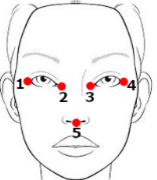
\includegraphics[width=0.3\textwidth]{figures/lmark.png}
    \caption{Os cinco pontos de landmark utilizados}
    \label{fig:lmark}
\end{figure}


\subsection{Parametros do Treinamento}
O treinamento de um modelo é definido pela configuração de uma série de parâmetros. A configuração deles determina o tamanho, a acurácia e a velocidade do modelo gerado. Assim, variamos alguns parâmetros criteriosamente selecionados.
Os parâmetros escolhidos do algoritmo foram:
\begin{itemize}
    \item \textbf{Tree Depth} --- Especifica a profundidade das árvores usadas em cada cascata. Para cada árvore, existem $2^n$ folhas, onde $n$ é a profundidade da árvore. Este parâmetro representa a "capacidade" do modelo. 

\item \textbf{Nu} --- É o parâmetro de regularização. Ele determina a capacidade do modelo de generalizar e aprender padrões em vez de dados fixos ensinados. Quanto mais próximo de 1, mais o algoritmo priorizará o aprendizado de dados fixos em vez dos padrões, aumentando a chance de over-fitting. Por outro lado, quanto mais próximo de 0, mais o algoritmo reconhecerá padrões em detrimento de dados fixos, diminuindo a chance de  over-fitting. 
Com valores mais baixos, o modelo precisa de muitas amostras de treinamento para ter um bom desempenho, o que pode ser um problema.

\item \textbf{Cascade Depth} --- É o número de cascatas usadas para treinar o modelo. 

\item \textbf{Feature Pool Size} --- Indica o número de pixels usados para gerar as features para as árvores aleatórias em cada cascata. Uma quantidade maior de pixels levará o algoritmo a ser mais robusto e preciso, mas a ser executado mais lentamente.

\item \textbf{Num Test Splits}--- É o número de features de divisão amostradas em cada nó. Esse parâmetro é responsável por selecionar as melhores features em cada cascata durante o processo de treinamento.
\end{itemize}

\subsection{Dados Utilizados}
Em uma primeira tentativa de treinamento, utilizamos a biblioteca de imagens iBug 300W dataset~\cite{300w}, que disponibiliza um total de 28.867 imagens, sendo que grande parte delas possui mais de uma face na mesma imagem, com 68 landmarks anotados em cada uma delas. O tempo de processamento não foi viável.
Assim, em uma segunda tentativa, utilizamos a biblioteca de imagens dlib 5-point face landmark~\footnote{http://dlib.net/files/data/}. Ela possui 7.198 imagens de faces diversificadas baixadas da internet Também provém dois arquivos XML destinados ao treinamento e ao teste do modelo contendo as informações das anotações de 5 landmarks para cada face.

\subsection{Treinamento}
O treinamento se deu utilizando variações dos parâmetros previamente descritos. Para isso, a configuração inicial foi definida como mostra a Tabela~\ref{tab:conf0}.

\begin{table}[]
    \centering
    \begin{tabular}{|cc|}
    \hline
    Parâmetro & Valor Inicial\\
    \hline
    Tree Depth & 2\\
    \hline
    Nu & 0.1\\
    \hline
    Cascade Depth & 5\\
    \hline
    Feature Pool Size & 150\\
    \hline
    Num Test Splits  & 20\\
    \hline      
    \end{tabular}
    \caption{Configuração inicial}
    \label{tab:conf0}
\end{table}

Após isso, foram realizados mais 10 treinamentos, onde apenas um parâmetro foi variado em cada um deles. Cada parâmetro foi variado em dois treinamentos, possuindo um valor menor do que o de referência em um deles e um maior no outro. Os treinamentos ficaram configurados como mostra a Tabela~\ref{tab:modelo}.
\begin{table}[]
    \centering
    \begin{tabular}{|cc|}
    \hline
    Nome do modelo & Parâmetro alterado\\
    \hline
    1a & Tree Depth = 1\\
    \hline
    1b & Tree Depth = 8\\
    \hline
    2a & Nu = 0.001\\
    \hline
    2b & Nu = 1\\
    \hline
    3a & Cascade Depth = 1\\
    \hline
    3b & Cascade Depth = 15\\
    \hline
    4a & Feature Pool Size = 30\\
    \hline
    4b & Feature Pool Size = 800\\
    \hline
    5a & Num Test Splits  = 2\\
    \hline
    5b & Num Test Splits  = 200\\
    \hline
    \end{tabular}
    \caption{Para cada configuração de modelo caracterizado pela primeira coluna, foi alterado o parâmetro da segunda coluna.}
    \label{tab:modelo}
\end{table}
Com todos os modelos treinados, comparamos o desempenho entre eles e disponibilizamos os resultados mais adiante.

Além disso, realizamos um segundo teste, após o modelo ser treinado, que consiste em avaliar a acurácia na prática. Para isso, utilizamos 10 imagens de pessoas conhecidas e outras 10 imagens, uma para cada pessoa, para comparação. Assim, utilizamos o modelo para obter o valor de similaridade entre as duas imagens da mesma pessoa e obter o grau de diferença entre elas (que deve ser baixo, dado que são a mesma pessoa).

%%*****************************************************************************
\section{Materiais e Métodos}

\subsection{Requisitos}
Para desenvolver a solução, utilizamos a linguagem de programação Python com o  interpretador Python 3.7. São necessárias, também, as seguintes bibliotecas para Python: OpenCV~\footnote{https://opencv.org/}, Numpy~\footnote{https://www.numpy.org/}, Face Recognition~\footnote{https://github.com/ageitgey/face\_recognition}. Também utilizamos a biblioteca dlib~\footnote{http://dlib.net} para C++, que possui uma API para Python.

\subsection{Treinamento}
O arquivo "treinamento.py" utilizado para treinar os modelos pode ser encontrado no diretório "Treinamento". Junto dele, se encontra o dataset utilizado.
Além dos testes realizados logo após o treinamento, também desenvolvemos um novo teste, onde verificamos a eficiência do modelo na prática. O script utilizado se encontra no diretório "Treinamento/Testes pós treinamento" com o nome "compara\_fotos.py".

\subsection{Resultados da execução}
Os resultados obtidos se encontram no diretório "Resultados", onde a subpasta "Resultados de cada modelo" traz informações dos parâmetros utilizados e do erro médio obtido. Já os resultados do segundo teste se encontram na pasta "Testes pós treinamento".

\subsection{Aplicações}
Também disponibilizamos um diretório "Aplicações", onde estão dois scripts que usam os modelos treinados na prática. 

O script "img\_rec" utiliza imagens previamente inseridas no diretório "known"para comparar com a foto desejada, que deve estar com o nome "test.jpg" no mesmo diretório do script. Assim, caso a foto possua alguma face que seja considerada como conhecida, o script irá desenhar um contorno com o nome da imagem conhecida correspondente.

Já o script "cam\_rec", assim como o anterior, utiliza imagens da pasta "known" para comparar. Entretanto, desta vez, captura em tempo real e processa imagens da câmera acoplada ao computador. Para ser feito em tempo viável, as imagens capturadas são diminuídas antes de serem processadas.

%%*****************************************************************************
\section{Resultados e Discussão}
Uma vez treinados, submetemos os modelos aos testes comparando as imagens treinadas com as originais e também comparamos com outras imagens não utilizadas no treinamento. Depois disso, podemos comparar os resultados de todos os modelos e os resultados quando ele são utilizados na prática para determinar o grau de semelhança entre duas imagens distintas de uma mesma pessoa. 
\subsection{Erro Médio Obtido}
No primeiro teste, o erro é a diferença da média euclidiana de todos os pontos da imagem originalmente marcada e do resultado obtido através do modelo. Assim, obtivemos os valores da Tabela~\ref{tab:results}.

\begin{table}[]
    \centering
    \begin{tabular}{|cc|}
    Modelo & Erro Médio \\
    \hline
    Referência (configuração inicial) & Treinamento: 6.645\\ 
    & Teste: 8.308\\ 
    \hline
    1a & Treinamento: 8.238\\ 
    & Teste: 9.812\\ 
    \hline 
    1b & Treinamento: 1.689\\ 
    & Teste: 5.267\\ 
    \hline 
    2a & Treinamento: 16.415\\ 
    & Teste: 19.633\\ 
    \hline 
    2b & Treinamento: 6.530\\ 
    & Teste: 8.333\\ 
    \hline 
    3a & Treinamento: 12.499\\ 
    & Teste: 15.253\\ 
    \hline 
    3b & Treinamento: 4.627\\ 
    & Teste: 5.740\\ 
    \hline 
    4a & Treinamento: 8.412\\ 
    & Teste: 10.124\\ 
    \hline 
    4b & Treinamento: 6.267\\ 
    & Teste: 7.615\\ 
    \hline 
    5a & Treinamento: 8.046\\ 
    & Teste: 9.564\\ 
    \hline 
    5b & Treinamento: 6.088\\ 
    & Teste: 7.353\\ 
    \hline 
    Modelo já treinado & Treinamento: 1.964\\ 
    fornecido pela biblioteca& Teste: 2.914\\ 
    \hline 
    \end{tabular}
    \caption{Resultado da execução da aplicação durante a fase de treino e a fase de testes}
    \label{tab:results}
\end{table}
nto, como possuímos um dataset bem diverso, conseguimos um resultado satisfatório ainda assim.

Os modelos 3a e 3b utilizam variações de Cascade Depth. Onde valores menores geram arquivos pequenos ao custo de uma menor precisão, enquanto valores maiores produzem maior acurácia ao custo de arquivos maiores (2,2 MB ante 147 KB de 3a).

Já os modelos 4a e 4b trabalham com variações no Feature Pool Size. É possível verificar que um valor maior, provoca uma precisão maior, dessa vez sem aumentar significativamente o tamanho do arquivo. Entretanto, o tempo de processamento aumenta consideravelmente conforme aumentamos o valor do parâmetro.

Por fim, os modelos 5a e 5b variam o Num Test Splits. Assim como no modelo anterior, quanto maior o valor, mais acurado o modelo. Dessa vez, o tamanho final do modelo fica até menor conforme aumentamos o valor. Sendo, dessa forma, uma boa opção quando queremos boa precisão e tamanho pequeno. Entretanto, aumentar o valor aumenta consideravelmente o tempo de processamento.

Para o segundo teste realizado, selecionamos o melhor modelo obtido, o pior, o modelo referência e o modelo padrão fornecido pela biblioteca. Assim obtivemos os resultados da Tabela~\ref{tab:results2} para as fotos das 10 pessoas escolhidas.
\begin{table}[]
    \centering
    \begin{tabular}{|ccc|}
    \hline
    Modelo & Acurácia & Erro Médio\\
    \hline
    Referência & ana - 0.401 &\\
    (configuração inicial) & fatima - 0.423  & \\
    & faustao - 0.466 & \\
    & gugu - 0.487 & \\
    & malandro - 0.379  & 0,4268\\
    & ratinho - 0.441 & \\
    & raul - 0.509  & \\
    & regina - 0.42 & \\
    & sonia - 0.371 & \\
    & xuxa - 0.471 & \\
    \hline
    1b & ana - 0.372 &\\
    & fatima - 0.457 & \\
    & faustao - 0.434 & \\
    & gugu - 0.463 & \\
    & malandro - 0.39 & 0,4238\\
    & ratinho - 0.398 & \\
    & raul - 0.457 & \\
    & regina - 0.415 & \\
    & sonia - 0.382 & \\
    & xuxa - 0.47 & \\
    \hline
    2a & ana - 0.522 &\\
    & fatima - 0.385 & \\
    & faustao - 0.465 & \\
    & gugu - 0.472 & \\
    & malandro - 0.36 & 0,4432\\
    & ratinho - 0.41 & \\
    & raul - 0.561 & \\
    & regina - 0.41 & \\
    & sonia - 0.399 & \\
    & xuxa - 0.448 & \\
    \hline
    Modelo já treinado & ana - 0.389 &\\
    fornecido pela biblioteca& fatima - 0.446 & \\
    & faustao - 0.446 & \\
    & gugu - 0.478 & 0,4336\\
    & malandro - 0.39 & \\
    & ratinho - 0.402 & \\
    & raul - 0.455 & \\
    & regina - 0.38 & \\
    & sonia - 0.416 & \\
    & xuxa - 0.494 & \\
\hline
    \end{tabular}
    \caption{Resultados para o teste 2 que usa fotos de 10 pessoas.}
    \label{tab:results2}
\end{table}
Esses não são valores percentuais, entretanto também podem ser considerados como melhores quanto mais próximo de 0. No geral, uma medida abaixo de 0.5 para fotos de uma mesma pessoa já é satisfatório.

\subsection{Limitações}
Como não possuímos máquinas robustas dedicadas ao treinamento dos modelos e nem GPU para processar os dados de forma mais eficiente, tivemos uma limitação de recursos que não nos permitiu utilizar um banco de imagens extremamente grande e nem uma quantidade grande de landmarks, além de limitar as possibilidades de configurações dos parâmetros do algoritmo. A Figura~\ref{fig:limit} demostra o tempo esperada para processar os dados da forma citada.

\begin{figure}
    \centering
    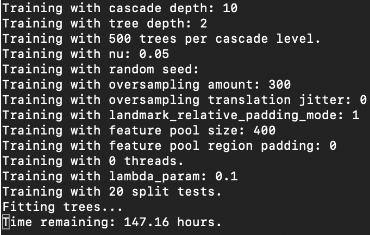
\includegraphics[width=0.5\textwidth]{figures/limit.png}
    \caption{Tentativa de processar um banco de imagens maior.}
    \label{fig:limit}
\end{figure}
Outra limitação está no uso do algoritmo para diversos fins, como o de reconhecer pessoas em uma rede social. Um site como o Facebook possui bilhões de usuários e comparar cada foto postada com todas as fotos de todos os usuários para reconhecer as pessoas presentes é absolutamente inviável, já que o resultado deve ser dado em milisegundos.

Uma terceira limitação está no limiar de corte para considerarmos duas fotos próximas o suficiente para ser a mesma pessoa. Aumentar o limite faz com que pessoas diferentes possam ser reconhecidas como a mesma. Diminuir, pode fazer duas fotos de uma mesma pessoa serem consideradas de duas pessoas diferentes.


%%*****************************************************************************
\section{Conclusões}
Os modelos treinados obtiveram resultados bem satisfatórios, tanto nos testes feitos após o treinamento quanto nos testes feitos com  aplicações na prática. Eles apresentam acurácia próxima do modelo fornecido por padrão com a biblioteca utilizada. Podemos verificar que mesmo o modelo menos eficiente ainda apresentou um ótimo resultado na prática.

Assim, chegamos a conclusão de que utilizando um banco de imagens de tamanho razoável e configurando os parâmetros sem exagerar nos valores, conseguimos facilmente um ótimo modelo com o algoritmo citado, mesmo possuindo poucos landmarks.

Verificamos ainda que podemos customizar e adequar o processo de treinamento do modelo de acordo com nossas necessidades, sejam elas de tempo de processamento, de tamanho de modelo ou de acurácia.


%%*****************************************************************************
%******************************************************************************
% Referências - Definidas no arquivo Relatorio.bib

\bibliographystyle{IEEEtran}

\bibliography{Relatorio}


%******************************************************************************




\end{document}
